% Emacs settings: -*-mode: latex; TeX-master: "manual.tex"; -*-

\chapter{Beam optical components:
Arms, slits, filters etc.}
This chapter contains a number of optical components
used to modify the x-ray beam in various ways,
as well as the ``generic'' component \textbf{Arm}.
\index{Library!Components!optics}
\index{Optics|textbf}

\section{Arm: The generic component}
\label{s:arm}
\index{Optics!Point in space (Arm, Optical bench)}
\mcdoccomp{Arm.parms}


The component \textbf{Arm} is empty; is resembles an optical bench
and has no effect on the xray.
The purpose of this component is only to provide a standard
means of defining a local coordinate system within the instrument definition.
Other components may then be
positioned relative to the \textbf{Arm} component
using the \MCX\ meta-language.
The use of \texttt{Arm} components in the instrument definitions
is not required but is recommended for clarity.
\textbf{Arm} has no input parameters.

The first Arm instance in an instrument definition may be changed into a
\verb+Progress_bar+(sec.~\ref{s:progress_bar}) component in order to display
simulation progress on the fly , and possibly save intermediate results.


\section{Slit: A beam defining diaphragm}
\label{s:slit}
\index{Optics!Slit}

\mcdoccomp{optics/Slit.parms}

The component \textbf{Slit} is a very simple construction.
It sets up an opening at $z=0$, and propagates the photon rays
onto this plane (by the kernel call PROP\_Z0).
Photons within the slit opening are unaffected,
while all other photons are discarded by the kernel call ABSORB.

By using \textbf{Slit}, some photons contributing to the background
in a real experiment will be neglected.
These are, for instance, the ones that scatter off the inner side
of the slit, penetrate the slit material, or clear the outer edges of the slit.

The opening of the slit is determined by specifying either a \textit{radius}, a
width (\textit{xwidth}) and a height (\textit{yheight}), or absolute limits in $x$
and $y$ (\textit{xmin, xmax, ymin, ymax}), in order of precedence.
If \textit{radius} is set, the opening is considered circular.

The slit component can also be used to discard insignificant 
({\em i.e.}\ very low weight)
 rays, that in some simulations may be very abundant and therefore
time consuming. If the optional parameter \textit{cut} is set, all
x-rays with $p<\mathit{cut}$ are ABSORB'ed.
This use is recommended in connection with \textbf{Virtual\_output}.

\textbf{Slit} may be used to model slit diffraction, thourgh judicious use of the resmapling
parameters: \textit{focus\_xw,focus\_yh, focus\_x0, focus\_y0}. The similarity in parameter
naming for sources (chapter~\ref{c:sources}) is intentional as computationally the processes are
the same. If present the focus parameters cause the ray to be regarded as a Huygens wave and a new direction
going towards the resampling window is computed. The resulting difference in phase gives rise to maxima and minima as expected.
This feature should be used with care: the further away from the optical
axis, the more statistics and finer binning is needed to get meaningful results. Please refer to
~\cite{knudsen2013mcxtrace} for more deatils.



\section{Slit\_N: multiple slits}
\label{s:slit-n}
\mcdoccomp{optics/Slit_N.parms}

Documentation pending.


\section{Beamstop: A neutron absorbing area}
\label{beamstop}
\index{Optics!Beam stop}

%\component{Beamstop}{System}{$x_{min}$, $x_{max}$, $y_{min}$,
%$y_{max}$}{$r$}{}
\mcdoccomp{optics/Beamstop.parms}

The component {\bf Beamstop} can be seen as the reverse of
the {\bf Slit} component.
It sets up an area at the $z=0$ plane, and propagates the neutrons
onto this plane (by the kernel call PROP\_Z0).
Neutrons within this area are ABSORB'ed,
while all other neutrons are unaffected.

By using this component, some neutrons contributing to the background
in a real experiment will be neglected.
These are the ones that scatter off the side
of the beamstop, or penetrates the absorbing material.
Further, the holder of the beamstop is not simulated.

{\bf Beamstop} can be either circular or rectangular.
The input parameters of {\bf Beamstop} are the four coordinates,
$(x_{\rm min}, x_{\rm max}, y_{\rm min}, y_{\rm max})$
defining the opening of a rectangle, or the radius $r$ of
a circle, depending on which parameters are specified.

If the "direct beam" (e.g. after a monochromator or sample) should not be
simulated, it is possible to emulate an ideal beamstop 
so that only the scattered beam is left;
without the use of {\bf Beamstop}:
This method is useful for instance in the case where only neutrons 
scattered from a sample are of interest. 
The example below removes the direct beam and 
any background signal from other parts of the instrument
\begin{lstlisting}
COMPONENT MySample=V_sample(...) AT (...)
EXTEND
%{
  if (!SCATTERED) ABSORB;
%}
\end{lstlisting}


\section{Filter\_gen: A general filter using a transmission table}
\label{filter-gen}
\index{Optics!Filter}
\index{Sources!from 1D table input}

%\component{Filter\_gen}{System}{$x_{min}$, $x_{max}$, $y_{min}$, $y_{max}$, $file$}{$options$}{validated, flat filter}
\mcdoccomp{optics/Filter.parms}

This component is an ideal flat filter
that changes the neutron flux according to a 1D input table (text file).

{\bf Filter\_gen} may act as a source ($options$="set")
or a filter ($options$="multiply", default mode).
The table itself is a 2 column free format file which accept comment lines.
The first table column represents wavevector, energy, or wavelength,
as specified in the $options$ parameter,
whereas the second column is the transmission/weight modifier.

A usage example as a source would use
\verb+options="wavelength, set"+, if the first column in the data
is supposted to be $\lambda$ (in \AA ).
Another example using the component as a filter would be
\verb+options="energy, multiply"+ if the first column is $E$ (in meV).

The input parameters are the filter window size
$x_{min}$, $x_{max}$, $y_{min}$, $y_{max}$,
the behaviour specification string $options$ and the file to use $file$.
Additionally, rescaling can be made automatic with the $scaling$
and relative $thickness$ parameters. If for instance the transmission data file
corresponds to a 5 cm thick filter, and one would like to simulate a 10 cm thick filter,
then use $thickness = 2$.

Some example data files are given with \MCS in the
\verb+MCSTAS/data+ directory as \verb+*.trm+ files for transmission.

\begin{table}
  \begin{center}
  {\let\my=\\
    \begin{tabular}{|l|p{0.7\textwidth}|}
    \hline
    File name & Description \\
    \hline
    Be.trm       & Berylium filter for cold neutron spectrometers (e.g. $k < 1.55$  \AA$^{-1}$) \\
    HOPG.trm     & Highly oriented pyrolithic graphite for $\lambda/2$ filtering (e.g. thermal beam at $k$ = 1.64, 2.662, and 4.1 \AA$^{-1}$) \\
    Sapphire.trm & Sapphire (Al$_2$O$_3$) filter for fast neutrons ($k > 6$ \AA$^{-1}$) \\
    \hline
    \end{tabular}
    \caption{Some transmission data files to be used with e.g. the Filter\_gen component}
    \label{t:source-params}
  }
  \end{center}
\end{table}

The filter geometry is a flat plane. A geometry with finite thickness can be simulated by
surrounding this component with two slits.


\section{Chopper\_simple: An ideal chopper}
\index{Optics!lens}
\mcdoccomp{optics/Chopper_simple.parms}
\texttt{Chopper\_simple} is an idelized version of a chopper with a rectangular chopper opening which may open
instantly and has no side-scattering etc.

It models the chopper with a blocking infinitely thin aperture which becomes transparent
in the time interval $t\in\left[\mathit{t0},\mathit{t0}+\tau\right]$.
This is an idelized version of a chopper where the chopper opening is rectangular which may open
instantly (if \textit{t\_rise}$=0$, the default). For nonzero rise time the aperture simply becomes gradually less opaque
for $t\in\left[\mathit{t0}-\textit{t\_rise},\mathit{t0}\right]$.

For correct normalization of intesity a chopper period, \textit{T}, must also be set.

\textit{is\_first} is useful when using \textbf{Chopper\_simple} with continous sources who inherently have no time-dependence. Thus the emission time of the photon
ray is arbitrary, and the chopper defines the temporal signature of the beam,
i.e. it simply sets the time-parameter of the photon ray randomly in the
opening window of the chopper. Naturally this should only be used for the \emph{first} chopper
element in a simulation.


\newpage
\chapter{Refractive optical components: lenses}
\label{c:lenses}

An X-ray refractive lens, often referred to as a Compund Refractive Lens (CRL), is a fairly new type of device, which has gained popularity in
the last few years. An early study showing the feasiblity of such devices may be found in~\cite{snigirev1996}. As the refractive index of X-rays
is $n\approx1$ a number of lenses, stacked together is usually necessary to bring the focal length to practical values. 
\MCX includes a few lens components, which all have slightly different charactertics.

\index{Optics|textbf}
%\section{Refractive lenses}
\label{s:lenses}
\index{Optics!Lens\_parab}

An X-ray refractive lens, often referred to as a Compund Refractive Lens (CRL), is a fairly new type of device, which has gained popularity in
the last few years. An early study showing the feasiblity of such devices may be found in~\cite{snigirev1996}. As the refractive index of X-rays
is $n\approx1$ a number of lenses, stacked together is usually necessary to bring the focal length to practical values. 
\MCX includes a few lens components, which all have slightly different charactertics.


\section{Lens\_simple: Thin lens approximation}
\label{s:lens-simple}
\index{Optics!lens}

\mcdoccomp{optics/Lens_simple.parms}

This models a thin-lens approximation of a stack of parabolic refractive x-ray lenses

\section{Lens\_parab: Thick parabolic CRL}
\label{s:lens-parab}
\index{Optics!lens}
\mcdoccomp{optics/Lens_parab.parms}

Component model of a stack of compund refractive lenses. Each lens in the stack
is modelled by two $2D$ parabolic surfaces, and rays are traced through all the
complete stack taking the displacement of the surfaces into account. This is
naturally less efficient than a thin lens approximation.

The logic behind the model is the following: a photon interacts with the
surface of the lens at a certain angle $\Theta$, which alters in accordance
with Snell's law upon photon's entering the lens's material. The combination of
the refractive process inside material (that is characterized by a material
datafile) and the interaction with a geometrical surface results in a photon's
new trajectory, i.e. in focusing.

The functionality of \texttt{Lens\_parab\_Cyl}, \texttt{Lens\_parab\_rough},
and \texttt{Lens\_parab\_Cyl\_rough} will be merged into this component.

\section{Lens\_parab\_Cyl: Thick 1D-parabolic CRL}
\label{s:lens-parab-cyl}
\index{Optics!lens}
\mcdoccomp{optics/Lens_parab_Cyl.parms}
This component is based on the same logical approach as the
\textbf{Lens\_parab} with one significant difference - geometrical surface.
Parabolic cylinder (parabolic curvature along the vertical axes only, invariant
along the horizontal) and thus ofocuses the beam in only in the vertical direction.

This component and its functionality is scheduled to be merged into \textbf{Lens\_parab}


\section{Lens\_parab\_rough: Thick parabolic CRL including roughness-model}
\index{Optics!lens}
\mcdoccomp{optics/Lens_parab_rough.parms}

This component and its functionality is scheduled to be merged into \texttt{Lens\_parab}

\section{Lens\_parab\_Cyl\_rough: Thick 1D-parabolic CRL including roughness-model}
\index{Optics!lens}
\mcdoccomp{optics/Lens_parab_Cyl_rough.parms}

This component and its functionality is scheduled to be merged into \texttt{Lens\_parab}


\section{Lens\_Kinoform: refractice kinoform lens}
\index{Optics!lens}
\mcdoccomp{optics/Lens_Kinoform.parms}

Doc. Pend.

\section{Lens\_elliptical: }
\index{Optics!lens}
\mcdoccomp{optics/Lens_elliptical.parms}

doc. pend.



\newpage
\chapter{Reflective optical components: mirrors}
\label{c:mirrors}
\index{Optics|textbf}
This section describes advanced reflective X-ray optics
components such as mirrors.
A description of the reflectivity of a mirror is found
in section~\ref{ss:mirrorreflect}.
%
\index{Optics|textbf}

This section describes advanced X-ray optics
components such as mirrors and analyzer crystals.
A description of the reflectivity of a mirror is found
in section~\ref{ss:mirrorreflect}.

\section{Mulitlayer\_elliptic: The elliptic multilayer mirror}
\label{s:mirror}
\index{Optics!Mirror plane}
\component{Multilayer\_elliptic}{System}{$\theta$, $s1$, $s2$, $length$, $width$, $R$}{}{validated}
%{$R_0, Q_c, W, \alpha, reflect$}{validated}

The component \textbf{Multilayer\_elliptic}
models a single rectangular reflecting multilayer mirror plate with elliptical curvature. It can be used
as a sample component, to \textit{e.g.}~assemble a Kirkpatrick-Baez focusing system 
or in combination with a double-crystal monochromator.


Figure~\ref{fig:Ellipse}\emph{Left} shows a side view of a mirror
(the blue section of the ellipse) in the McXtrace coordinate system.
At the mirror center, the mirror tangent is parallel to the $z$ axis
and the mirror normal is parallel to the $y$ axis. The width of the
mirror is $w$ and in $y-z$ plane the mirror has the curvature of an
ellipse with major axis $a$ and minor axis $b$,
%
\begin{equation} 
\frac{z^2}{ a^2} + \frac{y^2}{b^2} =1\,, \,|x| <
\frac{w}{2}\,.
\end{equation}
%
The length of the mirror is $L$. The coordinates of the mirror
center $(0,Y_0,Z_0)$ and the ellipse parameters $a$, $b$ are
determined uniquely by the central glancing angle, the source-mirror
distance and the mirror-image distance. The position of the mirror
is chosen to be at the positive side of the $y$ axis.

The input parameters of this component are:
$\theta$ [$^{\circ}$], the incident angle; 
$s1$ [m], the distance from the source to the multilayer;
$s2$ [m], the focusing distance of the multilayer;
$length$ [m], the length of the mirrors;
$width$ [m], the width of the mirror along the $x$-axis;
$R$, the reflectivity.

\subsection{Definition of the reference frames}
The direction and position of the incoming photon is defined
relative to the coordinate system illustrated in
Fig.~\ref{fig:Ellipse}\emph{Left} (in the code referred to as
\emph{McXtrace coordinate system}):
\begin{itemize}
\item the y-axis is parallel to the central mirror normal
\item the z-axis is parallel to the central mirror tangent
\item the origin is at the mirror center
\end{itemize}

However, all the calculations are conducted in another reference
frame which is illustrated in Fig.~\ref{fig:Ellipse}~\emph{Right}(in
the following referred to as the \emph{Ellipse coordinate system}):
\begin{itemize}
\item the z-axis is parallel to major axis of ellipse
\item the y-axis is parallel to minor axis of ellipse
\item the origin is at the center of the ellipse
\item the mirror center at $(0,Y_0,Z_0)$, uniquely determined by the
glancing angle at the mirror center, the source-mirror distance and
mirror-image distance.
\end{itemize}

\begin{figure}[htb!]
\centering
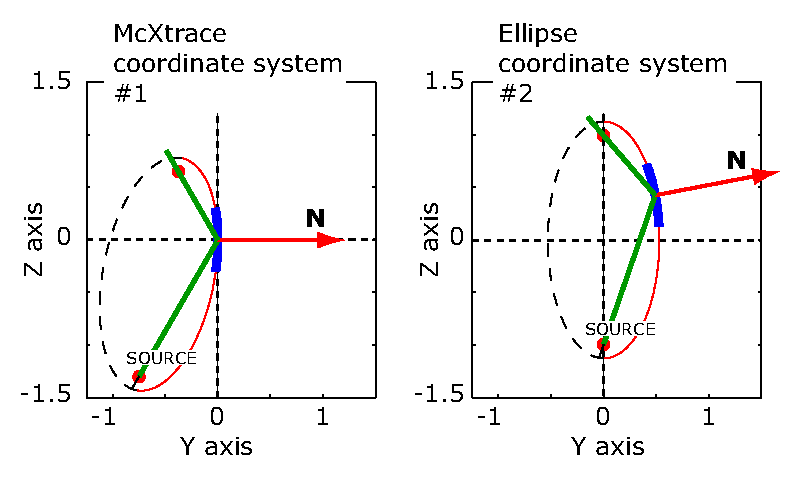
\includegraphics[width=0.95\linewidth]{figures/ellipse.eps}
 \caption{The same image in different coordinate systems.\newline \emph{Left}:
 \emph{McXtrace System} with the y-axis is parallel to the central mirror normal, the z-axis
 is parallel to the central mirror tangent and the origin is at the mirror
 center. \newline
 \emph{Right}: \emph{Ellipse System} with
the z-axis parallel to major axis of ellipse, the y-axis is parallel
to minor axis of ellipse and the origin is at the center of the
ellipse. }\label{fig:Ellipse}
\end{figure}


\subsection{Algorithm}
\begin{enumerate}
\item The photon is generated with a starting point $\bf{S}$ and a direction
$\bf{V}_\textrm{in}$ defined in the \emph{McXtrace} coordinate
system.
\item All calculations are performed in the \emph{Ellipse} coordinate system,
so to proceed the basis is changed to that reference frame.
\item The 2 intersections of the ray with the ellipse are determined.
\item It is checked if any of the intersections are within the area
defined by the mirror.
\item If one of the solutions is valid, the reflection of that ray is
determined.
\item The coordinates of the starting point and direction of the
reflected ray are calculated using the basis of the \emph{McXtrace}
coordinate system.
\end{enumerate}


\section{Reflection of the ray in the mirror}
\begin{figure}[htb!]
\centering
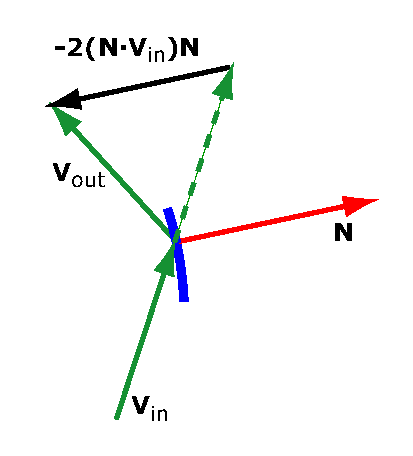
\includegraphics[width=0.3\linewidth]{figures/Dotproduct.eps}
 \caption{The reflection of the unit vector $\bf{V}_\textrm{in}$ in the mirror with the normal unit
 vector $\boldsymbol{{N}}$ is $\boldsymbol{{V}}_\textrm{out} = \boldsymbol{{V}}_\textrm{in} -2(\boldsymbol{{N}}\cdot\boldsymbol{{V}}_\textrm{in})\boldsymbol{{N}}$}\label{fig:dotProduct}
\end{figure}

The tangent and normal to the ellipse $z^2/a^2 + y^2/b^2=1$ at the
point $(Y,Z)$ are found by implicit differentiation: \begin{equation} 
\frac{2z}{a^2} + \frac{2y}{b^2} \,\frac{dy}{dz} = 0\,, \end{equation} so at the
point $(Y,Z)$ the slope of the tangent is $\frac{dy}{dz} =
-\frac{Z\,b^2}{Y\,a^2}$. The slope of the normal is minus the
inverse of the tangent slope, so the coordinates of the mirror
normal are \begin{equation} N_x = 0 \quad N_y = \frac{a^2\,Y}{b^2\,Z} \quad N_z =
1\,. \end{equation} With $\bf{V}_\textrm{in}$ and $\bf{N}$ denoting unit
vectors (direction and normal respectively), the direction of the
reflected ray is calculated as \begin{equation} \boldsymbol{{V}}_\textrm{out} =
\boldsymbol{{V}}_\textrm{in} -2(\boldsymbol{{N}}\cdot\boldsymbol{{V}}_\textrm{in})\boldsymbol{{N}} =
        \left(
      \begin{array}{c}
        V_{\textrm{in}x} - 2(\boldsymbol{{N}}\cdot\boldsymbol{{V}}_\textrm{in})N_x \\
               V_{\textrm{in}y} - 2(\boldsymbol{{N}}\cdot\boldsymbol{{V}}_\textrm{in})N_y \\
                V_{\textrm{in}z} - 2(\boldsymbol{{N}}\cdot\boldsymbol{{V}}_\textrm{in})N_z \\
      \end{array}
    \right)
\end{equation}


\subsection{Mirror reflectivity}
\label{ss:mirrorreflecttable}

At present, the Multilayer\_elliptic Mirror component uses a reflectivity table $reflect$, 
which 1st column is q [$\AA^{-1}$] and from the 2nd column on as the reflectivity $R$ in [0-1]
as function of tabulated energy [$KeV$]. 
An example file, calculated for a particular $Si/W$ multilayer, is provided (\verb+reflectivity.txt+).
User provided reflectivity data files can be parsed by the component.



\section{Mirror\_curved}
\label{mirror-curved}
\index{Mirror!Cylindrically curved mirror}
\component{Mirror\_curved}{System}{\textit{radius,length,width}}{\textit{coating,R0}}{}
 
Models a cylindrical mirror, positioned in the XZ-plane curving towards
positive X. The input parameter \textit{radius} defines the radius of curvature
and the mirror size is given by \textit{length} and \textit{width} where length
and width is along Z and Y respectively. \textit{coating} and \textit{R0} are mutually
exclusive. If \textit{R0} is nonzero, it is taken as the reflectivity value,
irrespective of wavelength, whereas coating nominates a file from which to read
values for $f_1$ and $f_2$. See~\cite{NIST-ffast} for definitions. For
elements $Z\in[1,92]$ datafiles are distributed with the McXtrace system that
may be used as: \verb+coating="Rh.txt"+. or \verb+coating="Al.txt"+. 

\section{Mirror\_curved: Cylindrically curved mirror}
\index{Optics!mirror}

\mcdoccomp{optics/Mirror_curved.parms}

A cylindrically curved mirror.
This component is scheduled to be merged with \texttt{Mirror\_parabolic} and \texttt{Mirror\_elliptic} 

\section{Mirror\_parabolic: Mirror with a parabolic curvature profile.}
\index{Optics!mirror}

\mcdoccomp{optics/Mirror_parabolic.parms}

This component is scheduled to be merged with \texttt{Mirror\_elliptic}

\section{Mirror\_elliptic: Mirror with a elliptic curvature profile.}
\index{Optics!mirror}

\mcdoccomp{optics/Mirror_elliptic.parms}

This component is scheduled to be merged with \texttt{Mirror\_parabolic}



\section{Multilayer\_elliptic: Elliptically curved mirror coated with a multilayer}
\label{s:mirror}
\index{Optics!multilayer, mirror}

\mcdoccomp{optics/Multilayer_elliptic.parms}

\index{Optics!Mirror plane}

The component \textbf{Multilayer\_elliptic}
models a single rectangular reflecting multilayer mirror plate with elliptical curvature. It can be used
as a sample component, to \textit{e.g.}~assemble a Kirkpatrick-Baez focusing system 
or in combination with a double-crystal monochromator.


Figure~\ref{fig:Ellipse}\emph{Left} shows a side view of a mirror
(the blue section of the ellipse) in the McXtrace coordinate system.
At the mirror center, the mirror tangent is parallel to the $z$ axis
and the mirror normal is parallel to the $y$ axis. The width of the
mirror is $w$ and in $y-z$ plane the mirror has the curvature of an
ellipse with major axis $a$ and minor axis $b$,
%
\begin{equation} 
\frac{z^2}{ a^2} + \frac{y^2}{b^2} =1\,, \,|x| <
\frac{w}{2}\,.
\end{equation}
%
The length of the mirror is $L$. The coordinates of the mirror
center $(0,Y_0,Z_0)$ and the ellipse parameters $a$, $b$ are
determined uniquely by the central glancing angle, the source-mirror
distance and the mirror-image distance. The position of the mirror
is chosen to be at the positive side of the $y$ axis.

The input parameters of this component are:
\textit{theta} [$^{\circ}$], the incident angle; 
\textit{s1} [m], the distance from the source to the multilayer;
\textit{s2} [m], the focusing distance of the multilayer;
\textit{length} [m], the length of the mirrors;
\textit{width} [m], the width of the mirror along the $x$-axis;
\textit{R}, the reflectivity.

\subsection{Definition of the reference frames}
The direction and position of the incoming photon is defined
relative to the coordinate system illustrated in
Fig.~\ref{fig:Ellipse}\emph{Left} (in the code referred to as
\emph{McXtrace coordinate system}):
\begin{itemize}
\item the y-axis is parallel to the central mirror normal
\item the z-axis is parallel to the central mirror tangent
\item the origin is at the mirror center
\end{itemize}

However, all the calculations are conducted in another reference
frame which is illustrated in Fig.~\ref{fig:Ellipse}~\emph{Right}(in
the following referred to as the \emph{Ellipse coordinate system}):
\begin{itemize}
\item the z-axis is parallel to major axis of ellipse
\item the y-axis is parallel to minor axis of ellipse
\item the origin is at the center of the ellipse
\item the mirror center at $(0,Y_0,Z_0)$, uniquely determined by the
glancing angle at the mirror center, the source-mirror distance and
mirror-image distance.
\end{itemize}

\begin{figure}[htb!]
\centering
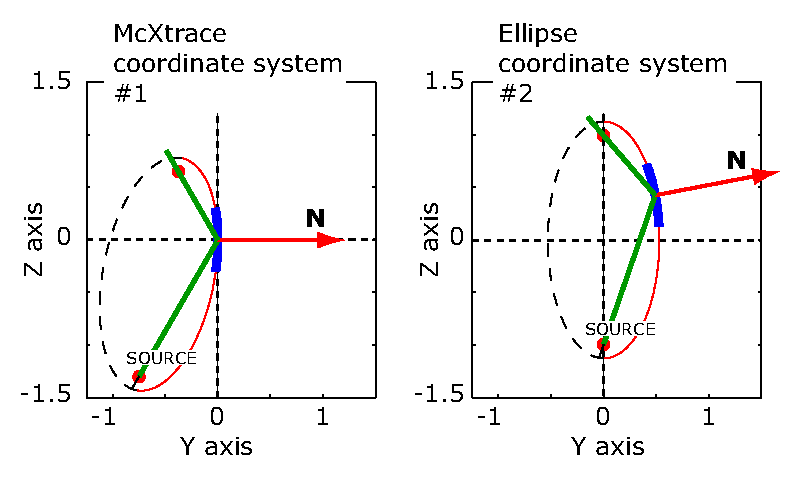
\includegraphics[width=0.95\linewidth]{figures/ellipse.eps}
 \caption{The same image in different coordinate systems.\newline \emph{Left}:
 \emph{McXtrace System} with the y-axis is parallel to the central mirror normal, the z-axis
 is parallel to the central mirror tangent and the origin is at the mirror
 center. \newline
 \emph{Right}: \emph{Ellipse System} with
the z-axis parallel to major axis of ellipse, the y-axis is parallel
to minor axis of ellipse and the origin is at the center of the
ellipse. }\label{fig:Ellipse}
\end{figure}


\subsection{Algorithm}
\begin{enumerate}
\item The photon is generated with a starting point $\mathbf{S}$ and a direction
$\mathbf{V}_\textrm{in}$ defined in the \emph{McXtrace} coordinate
system.
\item All calculations are performed in the \emph{Ellipse} coordinate system,
so to proceed the basis is changed to that reference frame.
\item The 2 intersections of the ray with the ellipse are determined.
\item It is checked if any of the intersections are within the area
defined by the mirror.
\item If one of the solutions is valid, the reflection of that ray is
determined.
\item The coordinates of the starting point and direction of the
reflected ray are calculated using the basis of the \emph{McXtrace}
coordinate system.
\end{enumerate}


\section{Reflection of the ray in the mirror}
\begin{figure}[htb!]
\centering
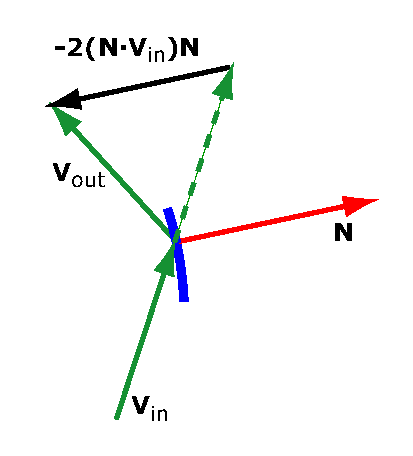
\includegraphics[width=0.3\linewidth]{figures/Dotproduct.eps}
 \caption{The reflection of the unit vector $\mathbf{V}_\textrm{in}$ in the mirror with the normal unit
 vector $\boldsymbol{{N}}$ is $\boldsymbol{{V}}_\textrm{out} = \boldsymbol{{V}}_\textrm{in} -2(\boldsymbol{{N}}\cdot\boldsymbol{{V}}_\textrm{in})\boldsymbol{{N}}$}\label{fig:dotProduct}
\end{figure}

The tangent and normal to the ellipse $z^2/a^2 + y^2/b^2=1$ at the
point $(Y,Z)$ are found by implicit differentiation: \begin{equation} 
\frac{2z}{a^2} + \frac{2y}{b^2} \,\frac{dy}{dz} = 0\,, \end{equation} so at the
point $(Y,Z)$ the slope of the tangent is $\frac{dy}{dz} =
-\frac{Z\,b^2}{Y\,a^2}$. The slope of the normal is minus the
inverse of the tangent slope, so the coordinates of the mirror
normal are \begin{equation} N_x = 0 \quad N_y = \frac{a^2\,Y}{b^2\,Z} \quad N_z =
1\,. \end{equation} With $\mathbf{V}_\textrm{in}$ and $\mathbf{N}$ denoting unit
vectors (direction and normal respectively), the direction of the
reflected ray is calculated as \begin{equation} \boldsymbol{{V}}_\textrm{out} =
\boldsymbol{{V}}_\textrm{in} -2(\boldsymbol{{N}}\cdot\boldsymbol{{V}}_\textrm{in})\boldsymbol{{N}} =
        \left(
      \begin{array}{c}
        V_{\textrm{in}x} - 2(\boldsymbol{{N}}\cdot\boldsymbol{{V}}_\textrm{in})N_x \\
               V_{\textrm{in}y} - 2(\boldsymbol{{N}}\cdot\boldsymbol{{V}}_\textrm{in})N_y \\
                V_{\textrm{in}z} - 2(\boldsymbol{{N}}\cdot\boldsymbol{{V}}_\textrm{in})N_z \\
      \end{array}
    \right)
\end{equation}


\subsection{Mirror reflectivity}
\label{ss:mirrorreflecttable}

At present, the Multilayer\_elliptic Mirror component uses a reflectivity table \textit{reflect}, 
which 1st column is q [$\AA^{-1}$] and from the 2nd column on as the reflectivity $R$ in [0-1]
as function of tabulated energy [\si{keV}]. 
An example file, calculated for a particular $Si/W$ multilayer, is provided (\verb+reflectivity.txt+).
User provided reflectivity data files can be parsed by the component.


\section{TwinKB\_ML: Side-by-side Kirkpatrick-Baez mirror pair}

\mcdoccomp{optics/TwinKB_ML.parms}

Models a pair of perpendicular, elliptically curved mirrors, known as a Montel-mirror or Side-by-side Kirkpatrick-Baez mirror.

